\chapter{\emph{Optimizing the Energy Efficiency}: Characterizing Wearable Usage In The Wild} \label{chap:wearable}



\section{Introduction}
\begin{table}[t]
\centering
\footnotesize
\begin{tabular}{c|l}
\multicolumn{1}{c|}{Topic}  & \multicolumn{1}{c}{Key Results} \\
\hline
 Device states & Dozing dominates the usage (50.6\%); wake-up accounts for 2\% of usage period; \\& wake-up sessions are short but frequent (72 per day on average) with various root \\& causes  such as ``flick and look'' and push notifications. \\
\hline
 Push notifications  & Push notifications are used by 200+ apps, dominated by IM/emails, and exhibiting \\& bursty arrival patterns.  \\
\hline
 Smartwatch apps     & A wide spectrum of watch apps are observed; their execution is dominated by short \\& background services. \\
\hline
 Power models        & Accurate and comprehensive power models for two popular watches. The models \\& have error rates $<$6\%. \\
\hline
 Energy utilization  & Dozing and wake-up account for 56\% and 27\% of overall energy respectively. At \\& component level, CPU (29\%) and display (30\%) dominate the energy consumption. \\& Network consumes only 3.4\% of the energy. \\
\hline
 Energy optimization & ``What-if'' analysis over real data for improving energy efficiency; impact of state \\& machine on battery drain. \\
\hline
 Network traffic     & Watches are paired with phones during 84\% of the daytime; most flows are small, \\& short, slow, and bursty. \\
\end{tabular}
%\vspace{-.1in}
\caption{\footnotesize Key results and findings of smartwatch study.}
%\vspace{-.1in}
\label{tab:toc}
\end{table}

Smartwatch carries numerous ``simplified'' mobile applications and it has become one of the most popular wearable computers on the market, it offers great convenience to end users through a wide range of
features such as receiving push notifications, issuing voice control,
monitoring fitness, and interacting with 3rd-party apps. Despite
its popularity, smartwatches are still relatively new to the
commercial mobile device family, and the research community
lacks a thorough understanding of the smartwatch ecosystem. 

Smartwatch is operating under tight energy budget, typically its battery capacity are 3 quarters less than that of a smartphone. The very first step towards optimizing its energy efficiency is to systematically understand its usage in the wild. We bridge the gap by conducting an IRB-approved crowd-sourced measurement study of smartwatches involving 27 users. We first demonstrate it is feasible to build
a self-contained and comprehensive measurement data collector
on today’s off-the-shelf Android smartwatches. The collector
transparently collects a wide range of usage data, network traffic,
and system events in realistic usage scenarios, with very low
runtime and energy overhead incurred. We then provide each
of the 27 users with a state-of-the-art smartwatch instrumented with
the data collector. Using a 106-day dataset collected from our participants, we conduct an in-depth characterization of three key
aspects of smartwatch usage “in the wild”: usage patterns, energy
consumption, and network traffic characteristics. This is to our
knowledge the most comprehensive and in-depth crowd-sourced
study of smartwatches. Our key measurement results consist of
the following.

\BULLET We characterize the smartwatch usage patterns. An Android
watch can stay in one of the four states with diverse power
characteristics: fully awake, dozing (with dimmed watch face
display and restricted system activity), sleeping (screen further
turned off), and charging. We find that smartwatch’s wake-up
period accounts for only 2\% of the overall usage period among
the four states. The wake-up sessions are not only short, but
also frequent (72 times per day on average). We then analyze
their triggering factors, which help us identify key usage scenarios
of a watch: short ``flick and look'' sessions (the most common
interaction type that the OS needs to be optimized for), push
notifications, longer interaction sessions, and unintended wake-up.

\BULLET A key usage scenario of smartwatches is to receive push
notifications. In our dataset, more than 200 apps send push
notifications to the watch through either the OS-provided Android
Wear service or custom data channels between phone-side and
watch-side apps. Push notifications are dominated by instant
messaging and emails. Despite a potential lack of long-term
predictability, push notifications’ arrival exhibits a strong bursty
pattern, with a median inter-arrival time of only 49 seconds. Also
there is room for the OS to improve push notification delivery, by
strategically determining whether to push and how to push.

\BULLET We also investigate how smartwatch applications (apps) behave.
We find smartwatch app execution is dominated by short but
frequent background services, whose total duration is more than
50 times longer than that of full-screen activities, which users
seldom launch due to a watch’s small form factor making fullfledged
interaction challenging. The services, together with the
OS infrastructures (\emph{e.g.}, the push notification and card management
subsystems) should therefore be the optimization focus for OS and
app developers.

\BULLET We derive comprehensive and accurate power models for two
popular Android smartwatches. We then apply the power
models to the user study data to quantify the energy consumption
of smartwatches in the wild. We made several interesting
observations. More than half of the smartwatch energy is consumed
by the dozing state (56\%) due to its long duration. Meanwhile, the
awake state also plays an important role in energy consumption
(27\%) despite its very short usage duration (2\%). Due to the
big power consumption gap between awake and dozing/sleeping,
a small increase of the wake-up duration will be ``amplified'' from
the battery draining perspective, thus shortening the standby time of
the watch. The top-2 energy-hungry components on smartwatches
are the same as those on smartphones: CPU and display. Despite
smartwatches’ small screen sizes, display still contributes to 30.2\%
of the overall energy. CPU accounts for 29.3\% of the overall
smartwatch energy. Network interfaces, however, consume a
very small fraction of energy on smartwatches without a cellular
interface.

\BULLET We investigate how to make smartwatches more energy-efficient
using combined approaches of trace-driven ``what-if'' analysis
and controlled in-lab experiments. Our results suggest that
the energy efficiency can be further improved through a wide
range of optimization strategies such as optimizing the display,
bundling delay-tolerant push notifications, and dynamically
configuring CPU’s online cores and frequencies. Also the watch’s
state machine and its associated timers affect the
energy consumption and need to be strategically determined, as
demonstrated by our ``what-if'' analysis. 

Our key measurement findings are listed in Table~\ref{tab:toc}. 
To summarize, the major contributions consist of the following.
\begin{itemize}
	\item We develop a self-contained and lightweight measurement data
	collection system for Android Wear smartwatches, and conduct a
	real deployment on 27 users.
	\item We derive accurate and comprehensive power models for two
	commodity Android Wear watches.
	\item We perform systematic measurements of smartwatches’ usage
	patterns, energy consumption profiles, and network traffic characteristics
	using a 106-day dataset collected from 27 users. Based on
	our findings, we identify key energy inefficiencies in the smartwatch ecosystems
	that can be further improved, and propose recommendations via trace driven ``what-if'' analysis.
\end{itemize}



\section{The Smartwatch User Study}
We launched an IRB-approved user study which is open to students, faculty, and staff members on our campus. We recruited 27
participants from more than 200 applicants.
%
Each user was provided with an LG Urbane watch, a high-end smartwatch as of early 2016 (cost $\sim$\$250 USD). It is equipped with a quad-core Cortex A7 processor, 4GB storage, 512MB memory, Wi-Fi, Bluetooth, and various sensors. The watch runs Android Wear OS 1.3, which is based on Android 5.1.1.

\begin{table}[t]
	\centering
	\footnotesize
	\begin{tabular}{l|l|l}
		\multicolumn{1}{c|}{Collected Data Item}   & \multicolumn{1}{|c}{Method$^*$} & \multicolumn{1}{|c}{Source} \\
		\hline
		Wi-Fi packet trace                       & E    & tcpdump \\ %Event triggered \\
		Bluetooth packet trace                   & E    & BT Snoop Logger\\ %Event triggered \\
		User input events                        & E    & /dev/input/ \\
		Voice control input event                & E    & Android Wear log \\ %Event triggered \\
		Device wakeup/doze/sleep                      & E    & Android Wear log \\
		Device charging                          & E    & Android Wear API \\ %Event triggered \\
		Card post                                & E    & Android Wear API \\
		App activity/service state               & E    & atrace \\  %(create/start/stop/pause/resume)
		%Others (\eg network change)              & E    & (misc.) \\ %Event triggered \\
		%\comment{Battery level}          & P (5mins) \\
		Installed apps list                      & P (1 hour) & /data/app/ \\ %Periodically, every 5 mins \\
		Screenshot                               & P (30 sec) & screencap \\ %Periodically, every 5 mins \\
		CPU utilization                          & P (1 sec)  & /proc/stat \\ %Periodically, every 1s \\
		Screen brightness level                  & P (5 sec)  & Android Wear API \\ %Event triggered \\
		\hline
		\multicolumn{3}{l}{$^*$E = event triggered callback; P (interval) = periodical polling}
	\end{tabular}
	\vspace{-.1in}
	\caption{\footnotesize Types of data collected in the user study.}
	\vspace{-.1in}
	\label{tab:data}
\end{table}

We developed our own, which collects a wide range of data listed in Table~\ref{tab:data} in the background. The data collector was written in Java and native C/C++ with about 6,500 LoC.
%
Note the collector only runs at the watch side (the watch is rooted) and does not require any change on users' smartphones (which are usually not rooted).
The collected data is automatically uploaded to our secure server over Wi-Fi at night when the watch is being charged.
The data collection and upload processes are completely transparent to users.
%
As listed in Table~\ref{tab:data},
most data items are collected using event-triggered callbacks, including network traffic (both packet header and payload), user input, card post\footnote{A \emph{card} is a UI element in Android Wear. It shows a piece of information (\eg an incoming text message) to the user.}, device status, application states, \etc
%
In addition, the data collector performs periodic polling for a limited amount of other information, with the polling intervals being carefully chosen to balance between the runtime overhead and data collection frequency.


\section{Smartwatch Power Models}
A prerequisite for fine-grained energy analysis is a \emph{power model}, which is a function $E(\vec{A})$ that maps $\vec{A}$, system activities and events directly measurable on the device, to their incurred energy and power consumption. In the literature, numerous studies have derived energy models for smartphones~\cite{zhang10, qian11_mobisys, huang12_mobisys, pathak11_eurosys, pathak12_eurosys, nika:www, chen15:mobicom}. Nevertheless, to our knowledge, no power model is publicly available for smartwatches whose energy consumption profiles are quite different. To fill this gap, we empirically derive accurate power models for today's off-the-shelf smartwatches.

To measure the watch's energy,
%
we extract a compatible battery interface, which is used as a connector between the watch and the Monsoon power monitor~\cite{monsoon}, from a same-vendor smartphone.
%
%we carved out a compatible battery interface circuit from a smartphone by the same vendor, and then used the interface circuit as an adapter between the watch and a Monsoon power monitor~\cite{monsoon}.
Our modeling approach follows the high-level methodology for smartphone power modeling~\cite{zhang10, chen15:mobicom, nika:www}.
When measuring a component, we keep other components offline (\eg Wi-Fi, BT, display) or at a steady power state (\eg CPU) whose power consumption is then subtracted from measured power value.
%
For components involving parameters (\eg CPU utilization), we programmatically change them and use regression to derive an empirical model as a function of the parameters.
We repeat each experiment 10 times and use the average power for modeling.
The overall watch power is then estimated as the sum all components' power consumption.

\begin{table*}[t]
\centering
    \begin{footnotesize}
				\begin{tabular}{l|l|l}
				\multicolumn{1}{c}{\MR{Component}}               & \multicolumn{2}{|c}{Power Consumption (mW) } \\ \cline{2-3}
				                             & \multicolumn{1}{c}{LG Urbane (user study)}    &   \multicolumn{1}{|c}{LG Watch R}             \\
				\hline
				Dozing base + display        &  24.3 (base 12.1 + display 12.2)              &   22.7 (base 10.7 + display 12.0)             \\
				%Dozing display               &  12.2                                         &   12.0                  \\
				%Doze (watch face off)       &  10.5 for the entire device                   &   10.8 for the entire device                  \\
				%Doze watch face display     &  12.2                                         &   11.9                                        \\
				Sleeping base                   &  14.5                                         &   17.6                                       \\
				Wake-up base                 &  47.1                                         &   54.9                                        \\
				\hline
				CPU                          &  $214.0u$, $u \in$ (0,1]: CPU util.           &   $216.2u$, $u \in$ (0,1]                     \\
				%\hline
				%Dozing display                 &  12.2                                         &   12.0 \\
				\hline
				\multicolumn{3}{l}{Wake-up display power = $\sum{(c_r \cdot r+c_g \cdot g+c_b \cdot b+C)/K}$, Per-pixel $r,g,b \in$} \\
				\multicolumn{3}{l}{[0, 255], K = 320*320. Values of \{$c_r$, $c_g$, $c_b$, $C$\} are listed below.} \\
				\hline
				Wake-up brightness 1        & \{.023, .060, .084, 67.2\}                    &   \{.014, .036, .092, 60.6\}                 \\
				Wake-up brightness 2        & \{.034, .071, .129, 67.2\}                    &   \{.027, .060, .126, 60.6\}                 \\
				Wake-up brightness 3        & \{.041, .092, .167, 67.2\}                    &   \{.029, .077, .159, 60.6\}                 \\
				Wake-up brightness 4        & \{.055, .120, .201, 67.2\}                    &   \{.044, .096, .210, 60.6\}                 \\
				Wake-up brightness 5        & \{.058, .144, .236, 67.2\}                    &   \{.065, .127, .255, 60.6\}                 \\
				Wake-up brightness 6        & \{.076, .179, .303, 67.2\}                    &   \{.077, .163, .325, 60.6\}                 \\
				\hline
				BT Tail                      & 4.77 sec, Power: 34.1                         &   4.00 sec, Power: 13.88           \\
				BT Data ($\sim$ 0.5m)        & Tx: 111.5, Rx: 117.2                          &   Tx: 103.0, Rx: 104.6                       \\
				BT Data ($\sim$ 5m)          & Tx: 132.9, Rx: 116.2                          &   Tx: 121.5, Rx:  97.3                       \\
				BT Data ($\sim$ 10m)         & Tx: 130.8, Rx: 113.9                          &   Tx: 120.9, Rx:  98.2                       \\
				BT Scan                      & 146.0                                         &   155.1                                       \\
				\hline
				Screen touch/swipe           & 198.9                                         &   182.3                                      \\
				\end{tabular}
    \end{footnotesize}
    			 \captionof{table}{\footnotesize Derived power models for LG Watch Urbane and LG Watch R.}
			\label{tab:model}
 %\vspace{-.1in}
\end{table*}


\begin{table}[t]
\centering
\footnotesize
\begin{tabular}{l|l}
\multicolumn{1}{c|}{Component}                    & \multicolumn{1}{c}{Power (mW)} \\
\hline
Wi-Fi Tail                   & 0.18 sec, Power: 121.2  \\
Wi-Fi Promotion              & 0.30 sec, Power: 242.5  \\
Wi-Fi Data (-42 dBm)         & Tx: 669.1, Rx: 378.5              \\
Wi-Fi Data (-55 dBm)         & Tx: 672.8, Rx: 343.0              \\
Wi-Fi Data (-65 dBm)         & Tx: 840.7, Rx: 341.8              \\
Wi-Fi Scan                   & 252.3                             \\
\end{tabular}
%\vspace{-.1in}
\caption{\footnotesize Wi-Fi power model for LG Urbane.}
%\vspace{-.1in}
\label{tab:wifi_power}
\end{table}




We study two commercial smartwatches: LG Urbane (used in our user study) and LG Watch R.
LG Watch R has a similar configuration compared to LG Urbane except that it does not have built-in Wi-Fi.
%We also attempted to profile several other watches such as Samsung Galaxy Gear Live, but encountered issues making it difficult to hook the watch to the power monitor while performing controlled experiments (\eg the watch has non-removable battery or does not have a wireless debugging interface).
%
%The Samsung Gear 2 watch is different in that it has a dual-core 1.0 GHz CPU, 512 MB memory, 4 GB storage, 1.63 inch AMOLED display, and Bluetooth. The two LG watches use Android Wear while SG2 employs Tizen~\cite{xxx} as the operating system. Tizen is a Linux-based OS widely used in mobile devices and consumer electronics.
%
Table~\ref{tab:model} presents our derived power models for the two watches.
We first highlight our findings for the LG Urbane watch.
The power consumption of each state (awake, dozing, and sleeping) consists of an almost-constant base power plus power consumption of other components such as CPU, display, and network interfaces.
%with its key components highlighted as follows.
(1) At the dozing state, the overall device power consumption is low (24.3 mW).
The watch face display power accounts for about half of the overall dozing power. Since the watch face display has low brightness and mostly dark colors, its power can be modeled using a constant value (about 12.2 mW).
(2)
At the sleeping state, the power consumption is even lower since the display is turned off.
%When the watch wakes up, its base power (47.1mW) is about 2 times of the base power consumed in sleeping mode.
%
Also note that the watch is equipped with a low-power movement sensor and a microphone, whose power consumption is included in the base power. Since they run in an ``ambient'' manner (\ie always-on), it is difficult for us to separate their individual power contributions.
%The power can be further reduced by turning off the watch face.
(3) The watch is equipped with a 1.3 inch 320x320 P-OLED display, whose power is determined by the brightness level and the pixel colors~\cite{dong09_dac, dong11_mobisys} when the watch is awake. We find that blue is the most energy-consuming color component, followed by green and then red. Note our model does take into account the circular shape of the watch display~\cite{miao16_hotmobile} since only the displayed pixels are counted.
(4) The CPU power is determined by three factors: the number of online cores, the frequency of each core, and the utilization of each core. The LG Urbane watch is equipped with a quad-core Qualcomm Cortex A7 processor. However, three of the cores are forced to be offline by the OS, and the clock of the only online core is fixed at 787 Mhz. This is a common practice on Android smartwatches~\cite{liu16_mobisys}. Therefore, the only factor affecting the power is the CPU utilization, and we find both are linearly correlated.
(5) The Bluetooth state machine consists of an idle and an active state. The state promotion takes negligible time, while the demotion from the active to the idle state is triggered by an inactivity timer (``tail time'') of 4.77s.
(6) We find that the capacitive touch input also incurs non-negligible power consumption.
%EERS: Energy Efficient Responsive Sleeping on Mobile Phones
(7) Table~\ref{tab:wifi_power} measures the Wi-Fi power model for LG Urbane. The Wi-Fi state machine is similar to that of smartphones~\cite{chen15:mobicom, nika:www}, except that we observe a non-trivial state promotion delay of 0.3s. Also, we find when the RSSI is lower than -70dBm, likely due to its small built-in antenna,  the watch has difficulty associating with the AP. For LG Watch R, as shown in Table~\ref{tab:model}, its power model is qualitatively similar to that of LG Urbane except that it does not have a Wi-Fi interface.



\section{Energy Consumption in the Wild}
We now apply the LG Urbane power model to our user study dataset, to quantify the energy consumption of smartwatches in realistic settings.

\begin{figure}[t]
	\footnotesize
	\centering
	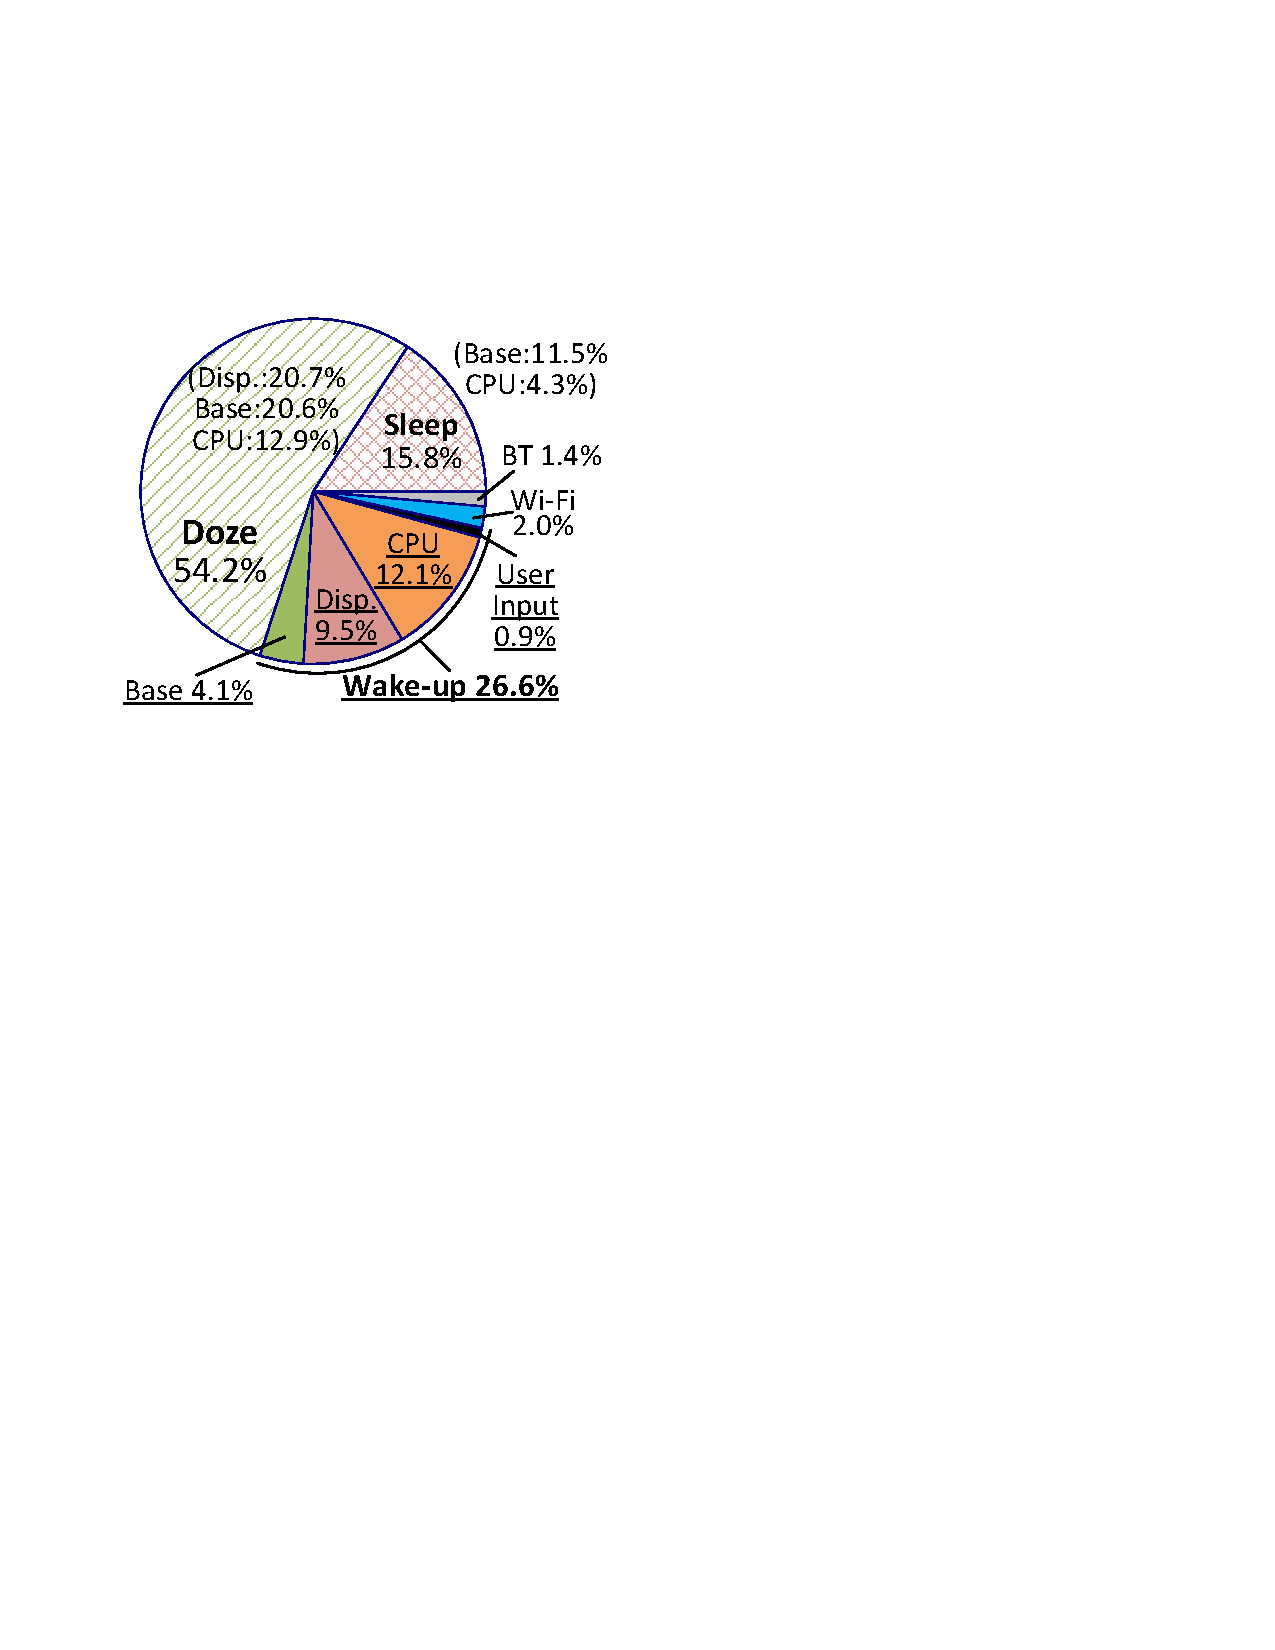
\includegraphics[width=.5\textwidth]{figs/smartwatch/energy_breakdown2.pdf} %\vspace{-2in}
	\caption{\footnotesize Component-level energy breakdown across all users.}
	\vspace{-.1in}
	\label{fig:energy}
\end{figure}

Figure~\ref{fig:energy} shows a more fine-grained energy breakdown. Within the dozing state, the energy consumed by the base, display, and CPU are roughly \{1.6:1.6:1\}. Despite its low brightness, display is still a key factor of battery drain when the watch is dozing. The dozing CPU energy comes from the maintenance window that periodically wakes up the CPU.
Within the awake state, display and CPU also dominate the energy consumption, accounting for 34.9\% and 44.5\% of the wake-up energy, respectively (or 9.5\% and 12.1\% of the overall energy respectively). The network incurs very small energy footprint (3.4\%). About 22\% of the Wi-Fi energy and 9\% of the Bluetooth energy are spent at the awake state (not shown in Figure~\ref{fig:energy}).

From Table~\ref{tab:model} and Figure~\ref{fig:energy}, we compute the average power consumption at the wakeup, dozing, and sleeping state to be 309.8mW, 31.9mW, and 14.5mW, respectively, across all users.
Note that the average dozing power (31.9mW) includes the base, the display, and the CPU power.
By weighing them using the usage duration breakdown, we can further compute the smartwatch's average power consumption to be 25.9mW across all states and users. Assuming that, a fully charged watch (with a battery capacity of 410 mAh for LG Urbane) can last for about 41.7 hours.


\section{Improving Smartwatch Energy Efficiency}
We study five methods for improving the smartwatch energy efficiency. We perform “what-if” analysis
on our dataset to reveal their impact on real smartwatch workloads
(or doing controlled experiments if a trace-driven analysis is not
feasible).

\textbf{1. Tuning the Awake$\rightarrow$Dozing Timer.} 

\textbf{2. Improving the Dozing$\rightarrow$Sleeping Mechanism.}

\textbf{3. Power-saving Color Transformation.}

\textbf{4. Bundling Delay-tolerant Push Notifications.} 

\textbf{5. Workload-aware CPU Configuration.}

Details for above 5 energy saving methods will be discussed during the proposal presentation.